
% top quark section 



In this section, we will review the  highlights of the top quark
program of linear colliders.     Since the top quark has not yet been
studied in $\ee$  reactions,  its study at a linear collider gives the
opportunity to dramatically improve the precision with which we know
its properties.   As we have explained above, such precision
measurement can reveal clues to the origin of the large mass of the
top quark and possibly, through this, to the nature of the Higgs
interactions that give mass to all fermions.
The potential of linear $e^+e^-$ colliders for top quark physics is
discussed in more detail in the 
ILC design reports~\cite{Baer:2013cma,Behnke:2013lya}
and in Refs.~\cite{Agashe:2013hma,Vos:2016til,Abramowicz:2018rjq}.




\subsection{Measurement of the top quark mass}
\label{subsec:top:topmass}

The top quark mass is a fundamental parameter of the Standard Model that must be
determined experimentally. Precise measurements are essential for precise tests of
the internal consistency of the Standard Model, through the electro-weak
fit~\cite{Baak:2014ora} or the extrapolation of the Higgs potential to
very high energy
scales~\cite{Degrassi:2012ry}.   The precise value of the top quark is
also needed as input to the theory of flavor-changing weak
decays~\cite{Buras:2009if} and models of the grand unification of the
fundamental interactions~\cite{Langacker:1994vf}.

The top quark pair production threshold was identified long ago~\cite{Gusken:1985nf} as
an ideal laboratory to measure the top quark mass, and other properties such as the top quark
width and the Yukawa coupling and the strong coupling constant~\cite{Strassler:1990nw}.
The large natural width of the top quark acts as an infrared cut-off,
rendering the threshold cross section insensitive to the non-perturbative confining part
of the QCD potential and allowing a well-defined  cross section
calculation within  perturbative QCD.  This calculation has now been
carried out the N$^3$LO order~\cite{Beneke:2015kwa} with  NNLL resummation~\cite{Hoang:2013uda}. Fully
differential results are available in WHIZARD~\cite{Bach:2017ggt}.

Given this precise theoretical understanding of the shape of the
$t\bar t$ threshold cross section as a function of center of mass
energy, it is possible to extract the value of the top quark mass by
scanning the values of  this cross section near threshold.  We
emphasize that the top quark mass determined in this way is, directly,
a short-distance quantity that is not subject to significant
nonperturbative corrections.
It is also closely related to the $\msb$ top quark mass, the input to
the theory calculations listed above. The uncertainty in the
conversion is less than 10~MeV~\cite{Marquard:2015qpa}.  This
contrasts with the situation at hadron colliders, where the
conversion uncertainties, the nonperturbative corrections, and the
experimental systematics in the measured top quark mass
contribute  independent uncertainties, each of which is about
200~MeV. 


\begin{figure}[tb]
 %\epsfysize=9.0cm
 \begin{center}
 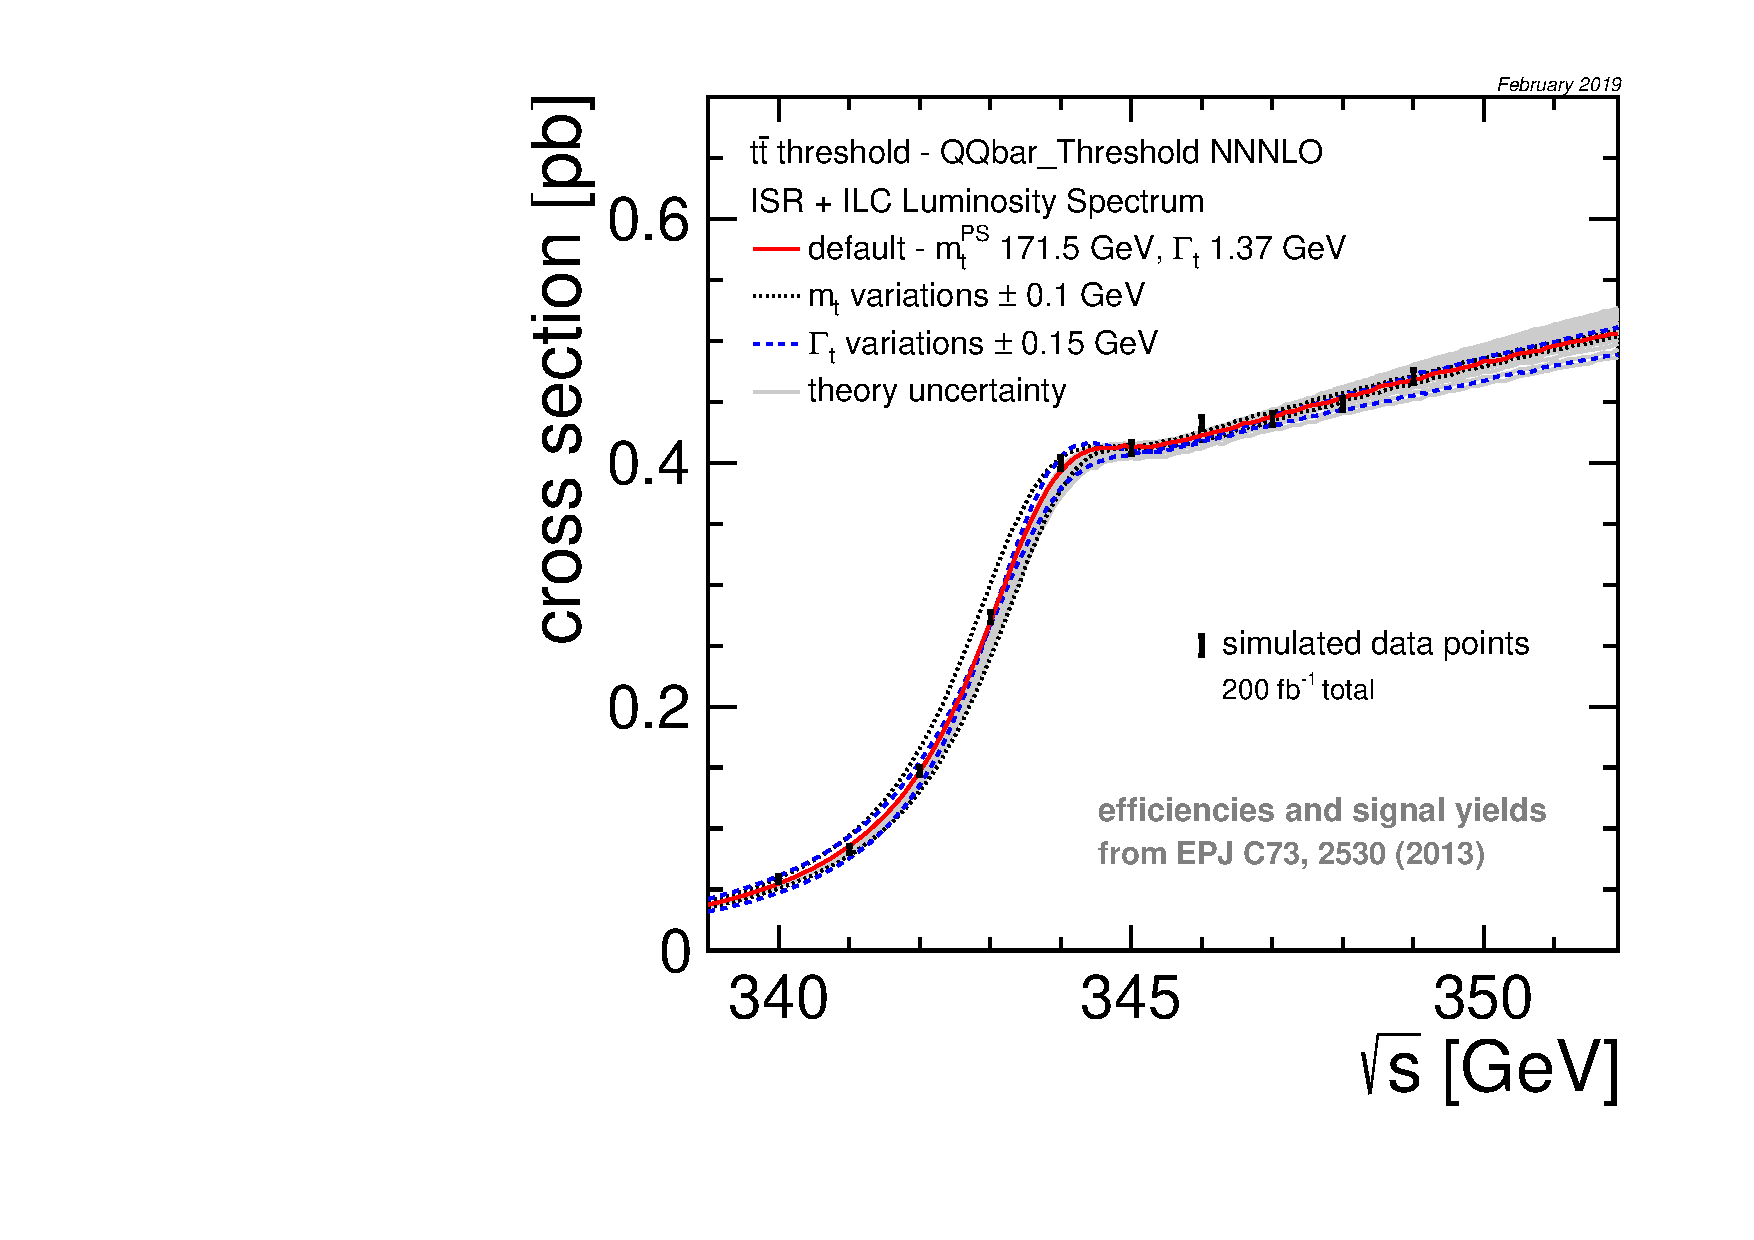
\includegraphics[width=0.8\hsize]{chapters/figures/thresholdscan_top_mass.pdf}
 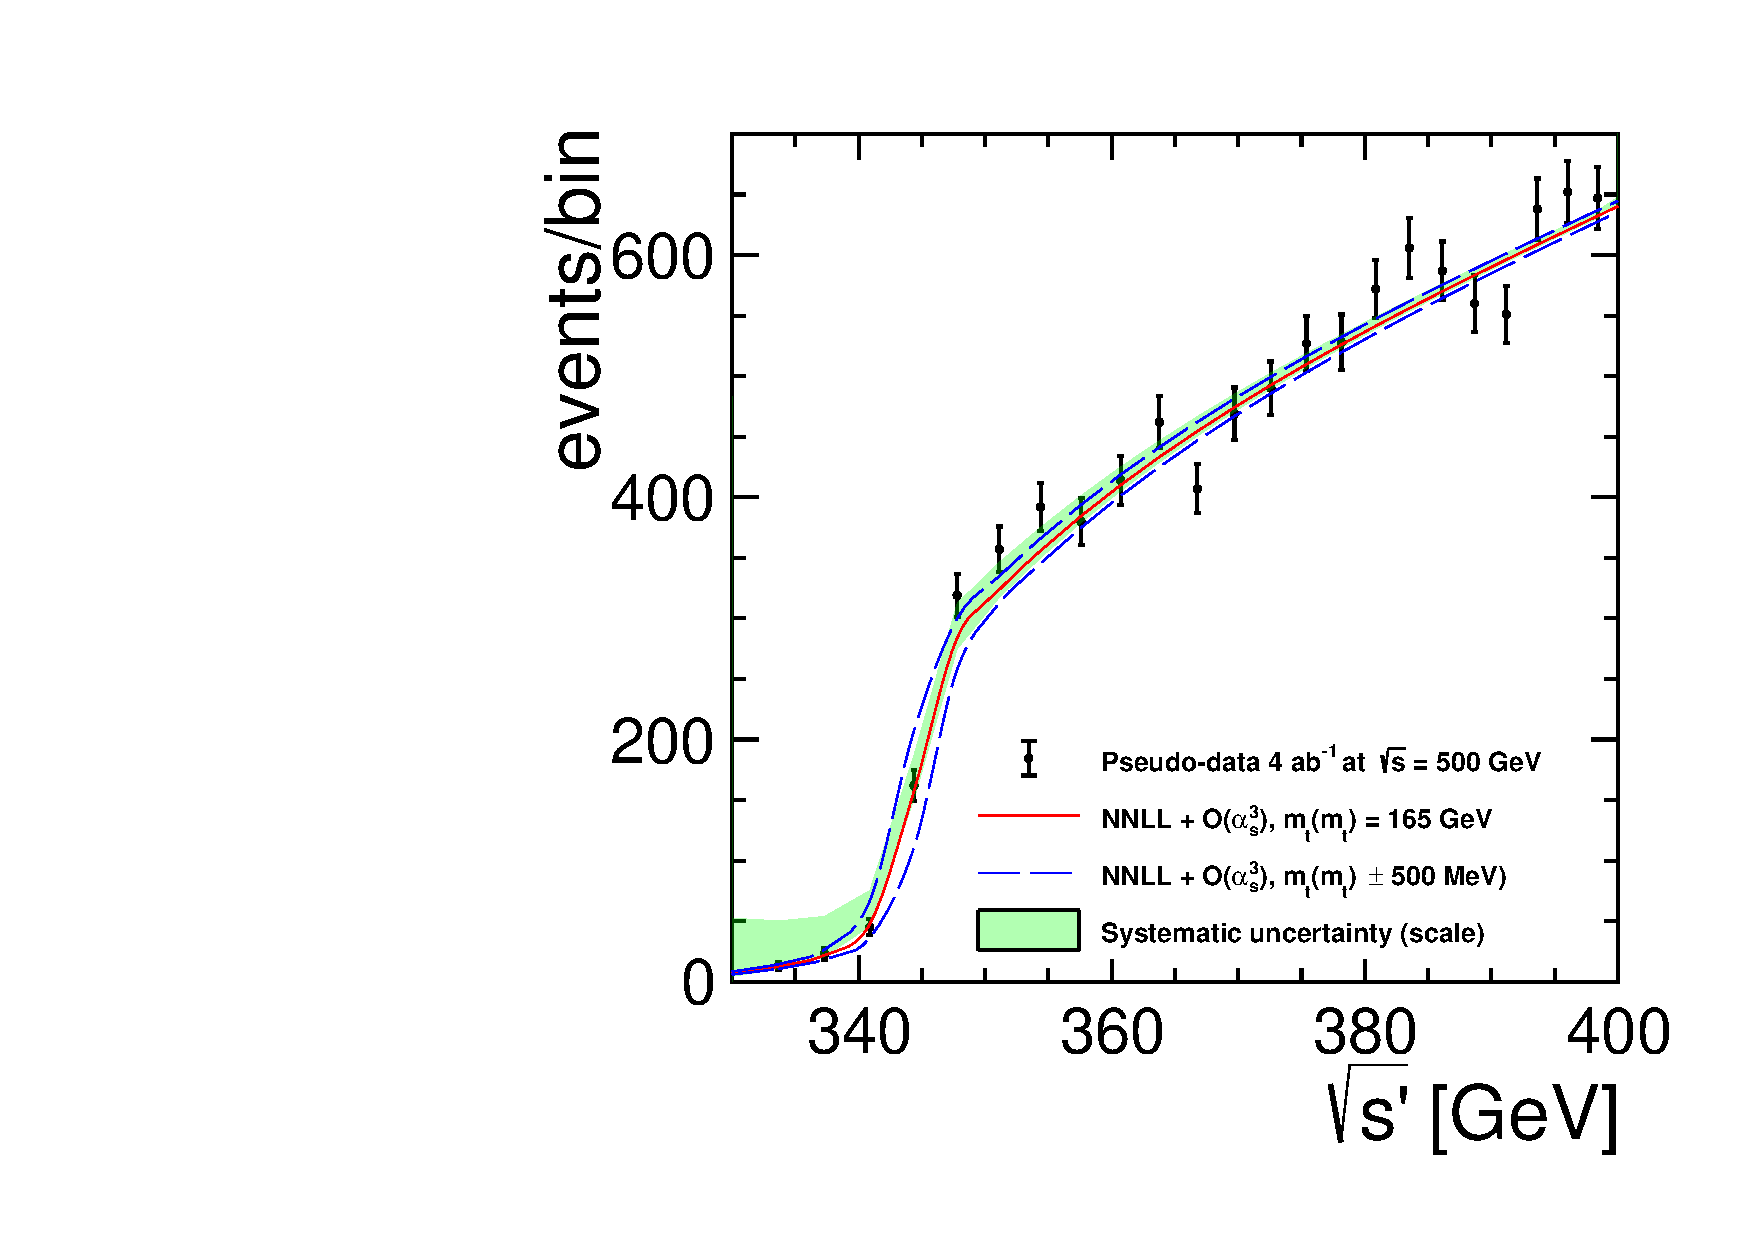
\includegraphics[width=0.8\hsize]{chapters/figures/alternative_top_mass.pdf}
\caption{Two methods to extract the top quark mass: (upper panel) a scan of the center of mass energy through the top quark pair production threshold, and (lower panel) a reconstruction of the differential $t\bar{t}\gamma$ cross section as a function of $s'$.
\label{fig:top_mass}}
 \end{center}
 \vspace{-0.7cm}
 \end{figure}
 


A simulation of the threshold scan is presented in
Fig.~\ref{fig:top_mass}. The scan of the $t\bar t$ threshold measures the
top quark pair production cross section at ten $e^+e^-$ center-of-mass energy points. 
The error bars on the pseudo-data point represent the statistical uncertainty of
the measurement, the uncertainty band indicates the theory (scale) uncertainty 
of the calculation. A fit of the line shape will give
a precise extraction of the top quark mass~\cite{Martinez:2002st,Horiguchi:2013wra,Seidel:2013sqa}.
The statistical uncertainty on the threshold mass is reduced to 
below 20~MeV with a scan of ten times 20~\ifb. The total uncertainty 
on the $\msb$ mass can be controlled to the level
of 50~MeV. These systematic uncertainties
include a rigorous evaluation of theory uncertainties in the 
threshold calculation and in the conversion
to the $\msb$ scheme~\cite{Simon:2016pwp}.

The top quark mass can also be measured precisely in operation above the $t\bar t$
threshold. The top quark mass can be extracted from the differential cross section of $t\bar t \gamma$ 
events as a function of the center of mass energy $\sqrt{s'} = \sqrt{s} ( 1 - \frac{E_{\gamma}}{\sqrt{s}})$ 
of the $t \bar t$ system of Fig.~\ref{fig:top_mass}. A fit with a calculation that matches the 
NNLL prediction for the threshold region with an $\mathcal{O} (\alpha_{s}^3)$ calculation for 
the continuum yields a total uncertainty of approximately 150~\MeV{}~\cite{Abramowicz:2018rjq}, 
including the statistical uncertainty and the theory uncertainty due to scale variations. A direct mass 
measurement can reach a statistical precision below 100~\MeV{}~\cite{Seidel:2013sqa} and will be helpful 
to clarify the interpretation of such measurements.

A linear $e^+e^-$ collider
can thus achieve a precision that goes well beyond
even the most optimistic scenarios for the evolution 
of the top quark mass measurement at the LHC.

\subsection{Searches for flavour changing neutral current interactions of the top quark}
\label{subsec:top:fcnc}

Among the direct searches for physics beyond the Standard Model with top quarks 
in the final state, the searches for flavour changing neutral current interactions of 
the top quark have been studied in most detail. Thanks to the excellent charm
tagging performance and the clean experimental environment such searches at the ILC
can compete with the sensitivity of the LHC to anomalous $ t Z c$, $t H c$ and 
$t\gamma c$ couplings. Searches for $e^+e^- \rightarrow t c$ production can
already be performed during the 250~\GeV{} stage~\cite{Hesari:2014eua}. Greater sensitivity can be achieved in searches for $t \rightarrow Hc$ and 
$t\rightarrow \gamma c$ decays above the $t\bar{t}$ production threshold.
Based on full-simulation studies~\cite{Zarnecki:2018wsw, Abramowicz:2018rjq} 
scaled to an integrated luminosity of 4~\iab{} 
at a center of mass energy of 500~\GeV{}{}, the 95\% C.L. limits on FCNC branching
ratios are expected to reach $BR(t \rightarrow Hc) \sim 3 \times 10^{-5}$ and 
$BR(t \rightarrow \gamma c) \sim 10^{-5}$, well in excess of the 
limits expected after 3~\iab{} at the HL-LHC. 


\subsection{Measurement of the top quark electroweak couplings}
\label{subsec:top:topelectroweak}

Composite Higgs models and models with extra dimensions naturally
predict  large corrections to the top quark couplings to the $Z$ and
$W$ bosons~\cite{Richard:2014upa,Barducci:2015aoa,Durieux:2018ekg}.
The study of top quark pair production at an $e^+e⁻$ therefore provide
a stringent test of such extensions of the SM.

The potential of the 500~GeV ILC for the measurement of the cross section and forward-backward asymmetry in
$t\bar{t}$ is characterized in detail in Ref.~\cite{Amjad:2015mma}. It
is important to note that these measurements search for deviations
from the SM in the main production mechanism of the $t\bar t$ system
through $s$-channel $\gamma$ and $Z$ exchange.   With two
configurations of the beam polarization, measurement of the angular
distribution, and measurement variables sensitive to the $t$ and $\bar
t$ polarizations, all 6 possible $CP$-conserving form factors can be
disentangled and constrained at the 1\% level. 
Especially designed $CP$-odd observables can also provide precise and
specific constraints on the $CP$-violating form factors~\cite{Bernreuther:2017cyi}. 
The expected 68\% C.L. limits on the form factors with 500~\ifb{} at
a center of mass energy of 500~\GeV{} are compared to the HL-LHC
expectation of Ref.~\cite{Baur:2004uw,Baur:2005wi} in Fig.~\ref{fig:top_ew_couplings}.

\begin{figure}[tb]
 %\epsfysize=9.0cm
 \begin{center}
 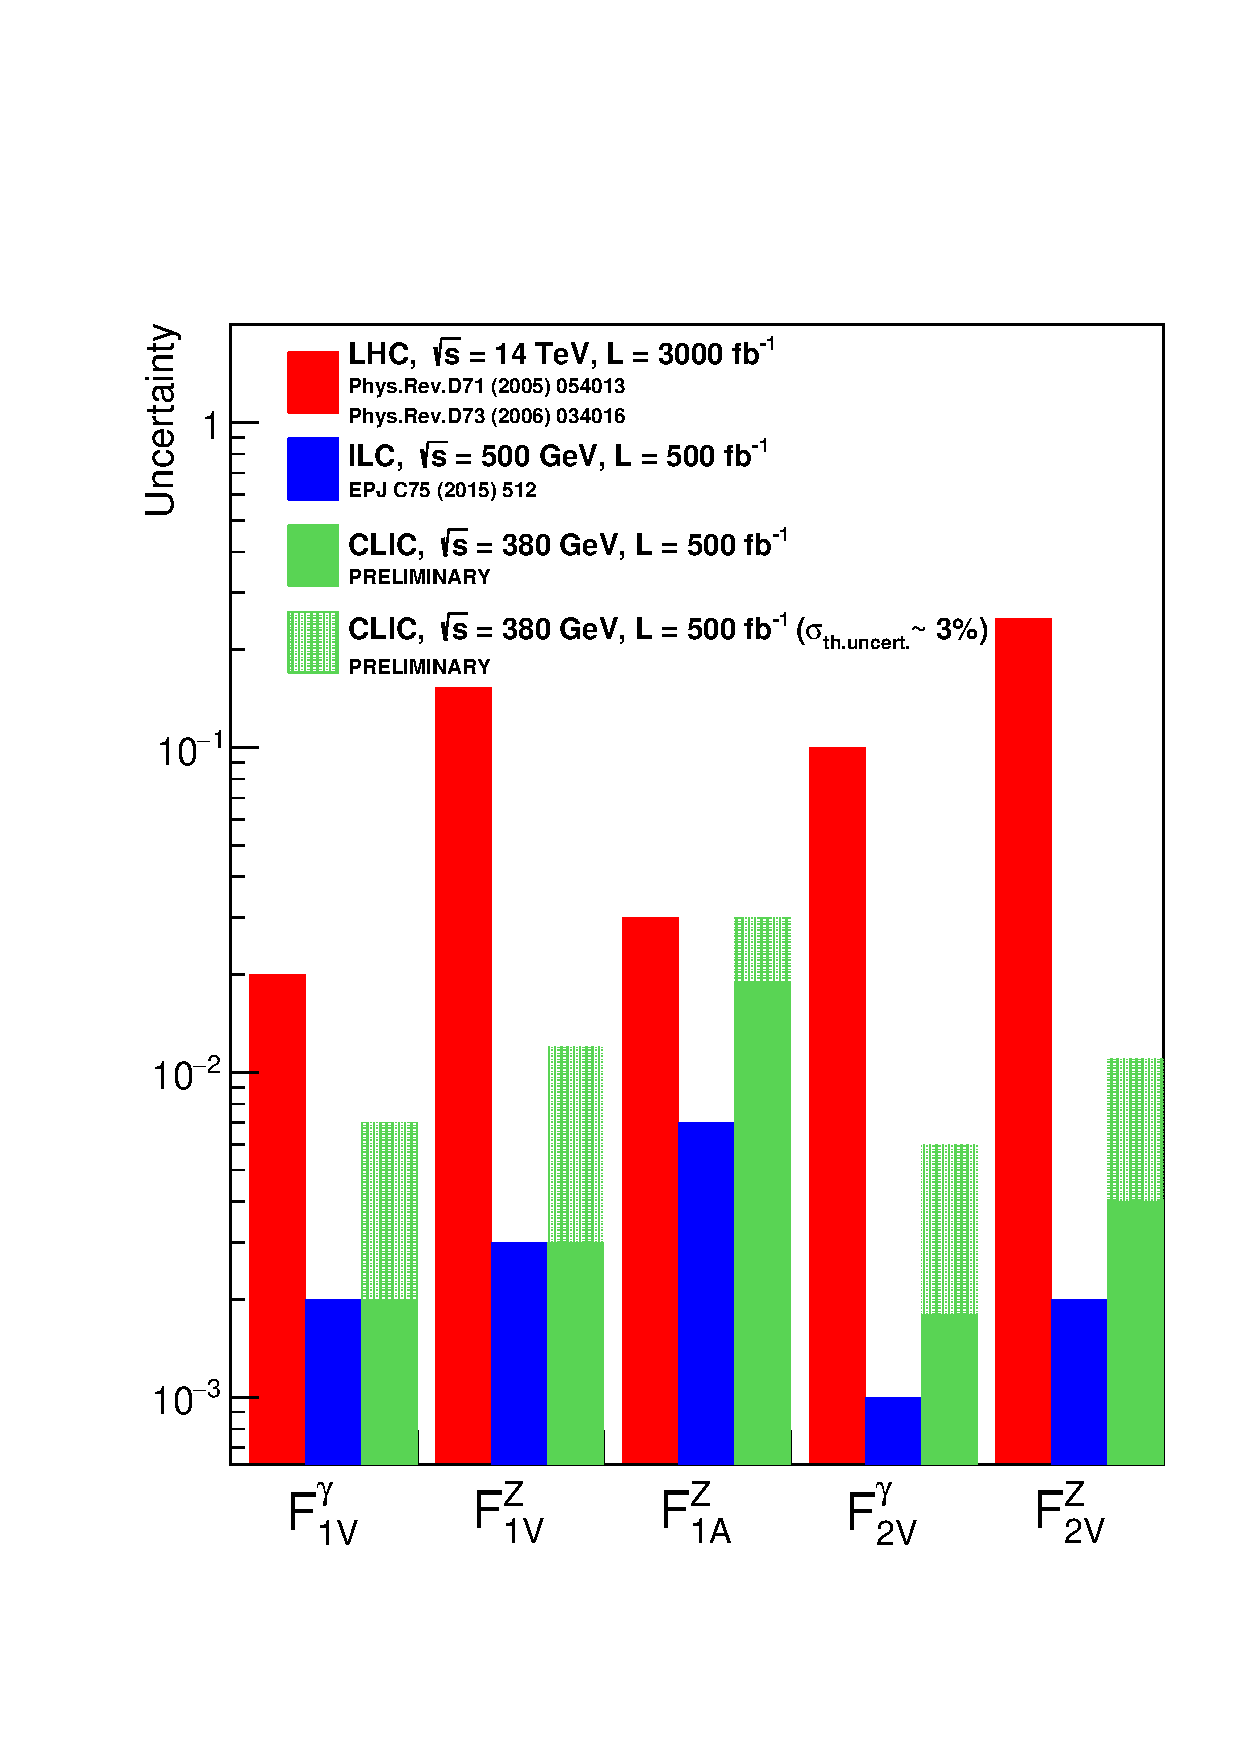
\includegraphics[width=0.8\hsize]{chapters/figures/top_ew_couplings_cpc.pdf}
 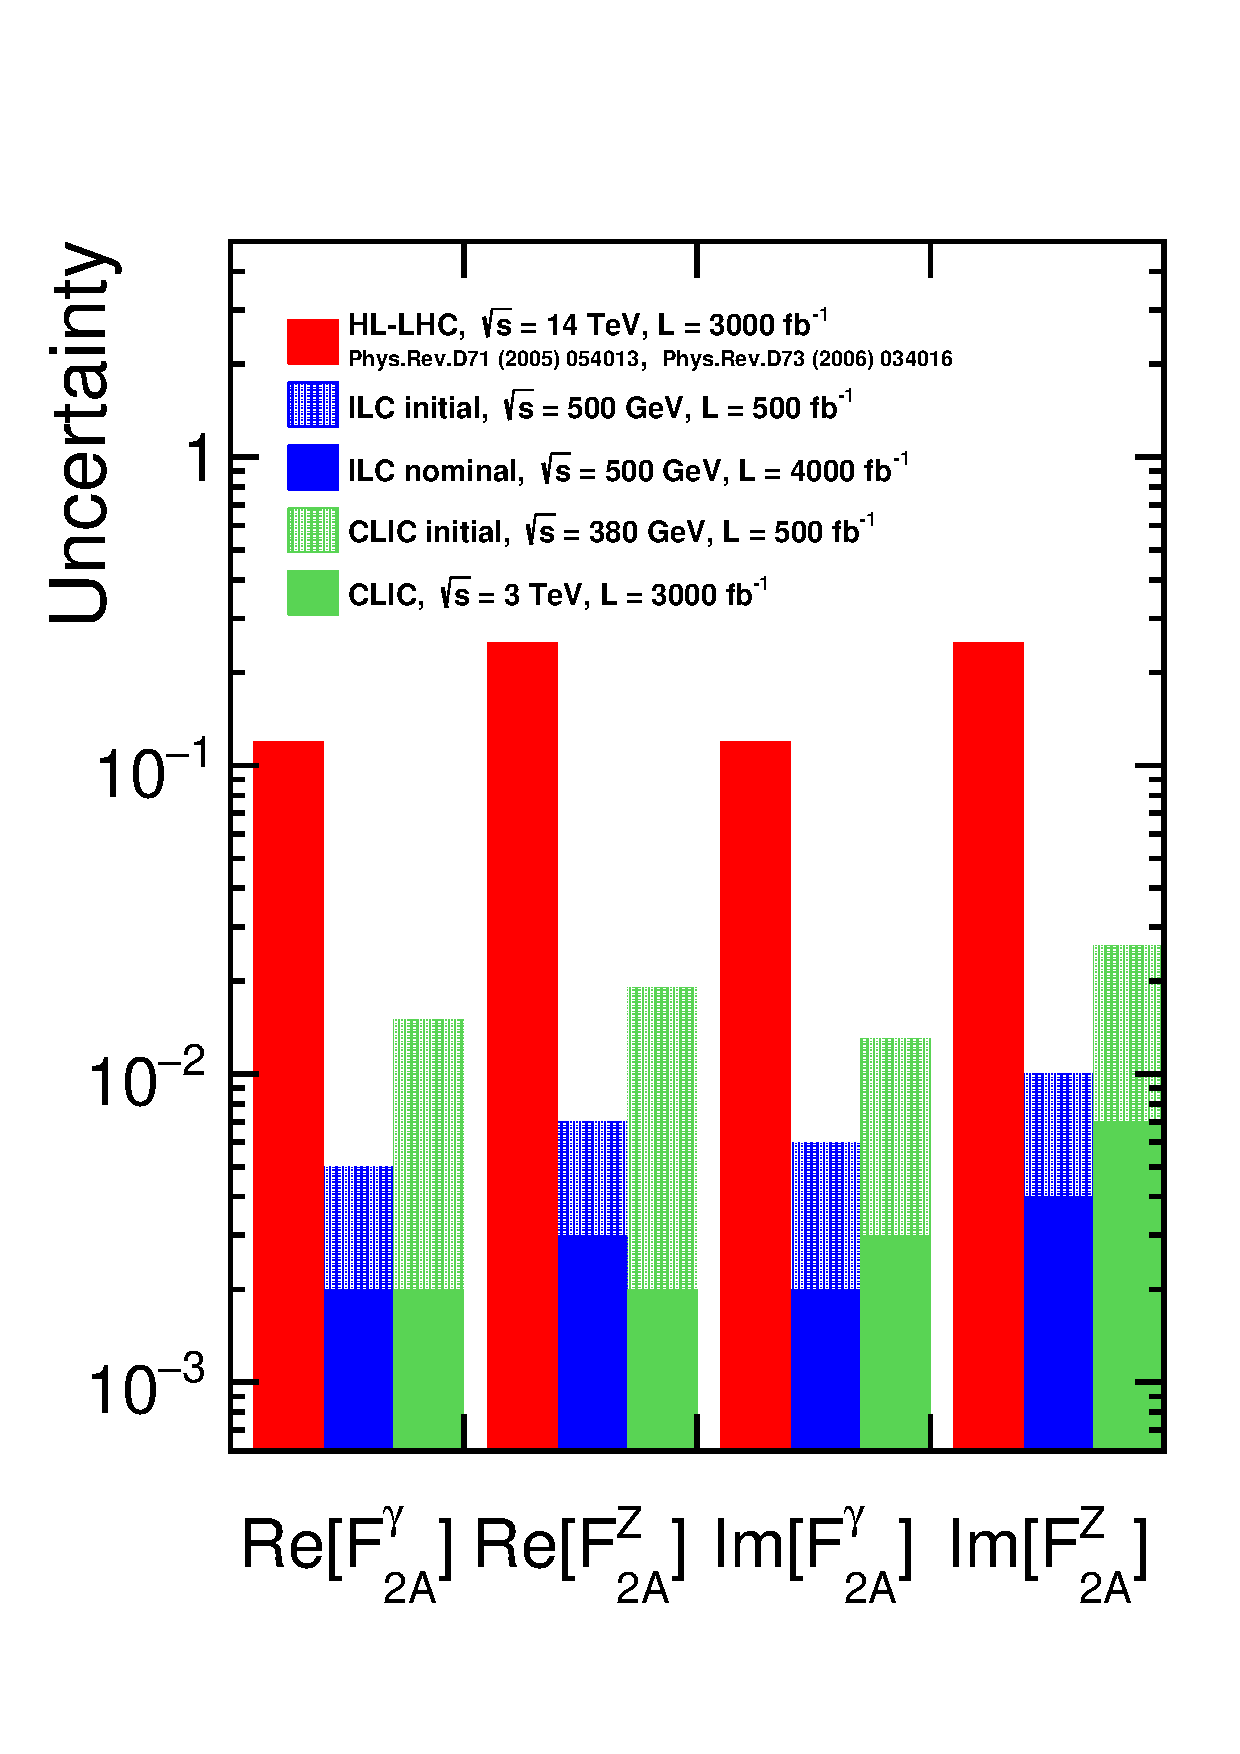
\includegraphics[width=0.8\hsize]{chapters/figures/top_ew_couplings_cpv.pdf}
\caption{The ILC prospects for the measurement of the electroweak couplings of the top quark, expressed as 68\% C.L. bounds on the form factors in a general expression 
for the Lagrangian that describes the $t\bar{t}Z$ and $t\bar{t}\gamma$ vertices:
(upper panel) CP-conserving form factors from Ref.~\cite{Abramowicz:2016zbo}, 
and (right) CP-violating form factors, from Ref.~\cite{Bernreuther:2017cyi}.
\label{fig:top_ew_couplings}}
 \end{center}
 \vspace{-0.7cm}
 \end{figure}
 

The corrections to the top quark electroweak couplings can 
be parametrized by set of 
dimension-6 operators of the SM EFT that contain the top quark as a
field. There is a large number of such operators, although the
restriction to $\ee$ reactions allows us to concentrate on a limited
set of operators that appear at the tree level in electroweak pair
production.
Because the top quark is massive, helicity conserving operators such
as chiral 4-fermion operators and helicity violating operators that
give corrections to the top quark magnetic moments must be considered
on an equal footing. 

In 
Ref.~\cite{Durieux:2018tev}, the authors consider the
perturbation of the reaction $\ee\to t\bar t$ by the 10 dimension-6
operators that contribute to the cross section at the tree level.
They show that a 
combination of
 the 500~GeV run, with excellent sensitivity to two-fermion operators,
with 1~TeV{} data, with increased sensitivity to four-fermion
operators, yields  tight constraints independently on 
all operator coefficients.  This study demonstrates the feasibility of a global EFT analysis of the top sector
at the ILC.  It also gives an the expected sensitivity of the ILC to
top electroweak couplings that  exceeds that of the HL-LHC programme by one to two orders of
magnitude. Translated into discovery potential for concrete BSM scenarios, a linear collider operated above the top quark
pair production threshold can probe for compositeness of the Higgs
sector to very high scales, up to 10~TeV and
beyond~\cite{Durieux:2018ekg}. 


Similar analyses, now requiring  only 4 relevant dimension-6 operator coefficients, can
improve the constraints on four-fermion operators involving $b$, $c$,
and light-fermion sectors beyond the results projected in
Sec.~\ref{subsec:ew_ffana}.

A combined fit of the operators relevant for the electroweak interactions of the
top quark.

\subsubsection{Measurement of the top quark Yukawa coupling coupling}
\label{subsec:top:topYukawa}


As with the trilinear Higgs coupling, the top quark Yukawa coupling can be
measured either directly or indirectly.  In the literature, most
estimates of the accuracy of determination of the top quark Yukawa
coupling are done within the simple context of the SM with only this
one parameter varied. We will quote uncertainties
within this model in this section and explore the implications of a general 
EFT analysis in Sec.~\ref{subsec:highE:top}.

Consider first the indirect determination of the top quark Yukawa coupling.
   For the Higgs boson decays
$H\to gg$, $H\to \gamma\gamma$, and $H\to Z \gamma$, there are no SM tree
diagrams
and so diagrams with top quark loops give leading contributions.  For
$h\to gg$, the top quark loop diagram gives the single largest
contribution.   In Tab.~\ref{tab:ILCLHC}, it is shown that the ILC
program up to 
500~GeV will determine the effective coupling in this process to bettter
than 1\%. Even higher precision can be obtained in a joint fit
including also the top quark radiative corrections to the cross
sections for $e^+e^- \rightarrow ZH$, $e^+e^- \rightarrow \nu\bar\nu
H$, and $e^+e^- \to  \gamma H$~\cite{Boselli:2018zxr}. However, one
should be uncomfortable that, for this determination, the simple model is
too simple, since new heavy colored particles can also contribute to
these processes at the 1-loop level. The indirect determination is 
sensitive to new physics in the $t\bar{t}h$ vertex, but does not provide 
a robust and unambiguous determination of the top quark Yukawa coupling. 
In a global EFT fit involving all relevant operators, the individual 68\% 
C.L. limit on $C_{\varphi t}$, but the marginalized constraint is ....

An indirect deterimination that calls out the top quark more
specifically is the measurement of the influence of the top quark
Yukawa coupling on the shape of the  $t\bar{t}$ pair production 
cross section very close to the $t\bar{t}$ threshold, due to the Higgs
boson-exchange contribution to the $t\bar t$ potential. In principle,
this effect could give a 4\% determination of the Yukawa coupling if
the QCD  theory of the top quark threshold region were precisely
known.   However, the Higgs-exchange effect is of the same size as
the N$^3$LO QCD corrections.  At this time, the threshold shape is
calculated only to this N$^3$LO order, by the use of a very sophisticated
NRQCD framework~\cite{Beneke:2015kwa}, combined with NNLL resummation of
large logarithms~\cite{Hoang:2013uda}.   Propagating the QCD
uncertainties gives an uncertainty of 20\% on the top quark Yukawa
coupling~\cite{Vos:2016til} , and there is no clear path at this time to improve the
accuracy of the QCD result.

 FInally, the top quark Yukawa coupling can be determined directly by
 measuring the cross section for the process $pp \rightarrow t\bar{t}h$ or
$e^+e^- \rightarrow t\bar{t}h$.  In the SM, these cross sections are simply
proportional to the square of the Yukawa coupling. The first measurements
of the $t\bar{t}h$ rate at the LHC~\cite{} yield a direct determination of 
the Yukawa coupling with an uncertainty of XXXX \%. The direct determination
from the $t\bar{t}h$ rate is expected

The cross 
section for $t\bar{t}h$ production increases rapidly above $\sqrt{s} \sim 500 $~GeV,
reaching several fb for $\sqrt{s} = 550$~GeV. Detailed studies of
selection
 and reconstruction of these complex multi-jet events
have been performed by the ILC at 500~GeV~\cite{Yonamine:2011jg} and
 1~TeV~\cite{Behnke:2013lya,Price:2014oca} and by CLIC
at 1.5~TeV~\cite{Abramowicz:2018rjq}. The direct measurement of the
top
 quark Yukawa coupling at the ILC reaches 3\%
precision~\cite{Fujii:2015jha}, with 4~\iab{} at 550~GeV.  With a sample of
2.5~\iab\  at 
1~TeV, this precision would improve to 2\%~\cite{Asner:2013psa}.  From
the energy-dependence of the cross section and the top polarizations,
this reaction can also be used to probe for non-standard forms of the
$tth$ coupling~\cite{Han:1999xd}.

In principle, the corrections to the top quark electroweak couplings
and to the top quark Yukawa coupling should be parametrized by
dimension-6 operators of the SM EFT.   Just as in the case of the
trilinear Higgs coupling, vertices arising from dimension-6 operators
that do not directly involve the Higgs boson can affect the cross
section for $\ee\to t\bar t H$ and thus create ambiguity in the
extraction of the top quark Yukawa coupling.   In $\ee to t\bar t H$,
the EFT corrections come from 4-fermion $eett$ operators and from
operators that correct the $\gamma$ and $Z$ anomalous moments of the
$t$ quark.   Similarly, in hadron-hadron collisions, the cross section
for $gg\to t\bar t H$ is corrected by dimension-6 operator that alter
the top quark vector coupling to gluons and those which create a
possible axial vector coupling to gluons and a gluonic magnetic
moment.  To extract the top quark Yukawa coupling in a
model-independent way, as opposed to the simple model used in
Sec.~\ref{subsubsec:highE:topYukawa}, the relevant EFT coefficients
need to be measured systematically in other top quark reactions.
Though we have indicated at the end of
Sec.~\ref{subsubsec:highE:topelectroweak} that such an analysis is
possible, the extraction from data of the EFT coefficient that shifts
the top quark Yukawa coupling has not yet been studied in simulations.